\documentclass[12pt,oneside]{article}
\usepackage[letterpaper,left=1in,right=1in,top=1in,bottom=1in]{geometry}
\usepackage{graphicx}
\begin{document}
\pagenumbering{gobble}
{
\centering
\Large
{
\textbf{
Crafting Adversarial Text Samples for Recurrent Neural Networks Using Windowed Inference and Search}
}
\vskip 9pt
by\\
Cory Nezin

\vskip 9pt
Professor Fred L. Fontaine, Advisor
{
\centering
\section*{Abstract}
}
}
\noindent
Neural networks have recently been found vulnerable to ``attacks'' which cause them to misclassify samples that were given a very small disturbance.  Attacks based on iterative gradient methods have been largely studied for numerically valued data like images.  In this work two new algorithms are described which extend the same kind of results to text.  One algorithm, ``window search'', does not require a continuous or differentiable model.  The other algorithm, ``gradient assisted window search'', is a hybrid algorithm which exploits word2vec based gradients for fast search.  The hybrid algorithm uses the gradient as a guide for candidate word replacements, and then performs an exponential search to determine the minimum number of replacements required to alter the classification of a text sample.  The algorithm is tested under white box, gray box, and black box scenarios.
\begin{figure}[h]
    \centering
    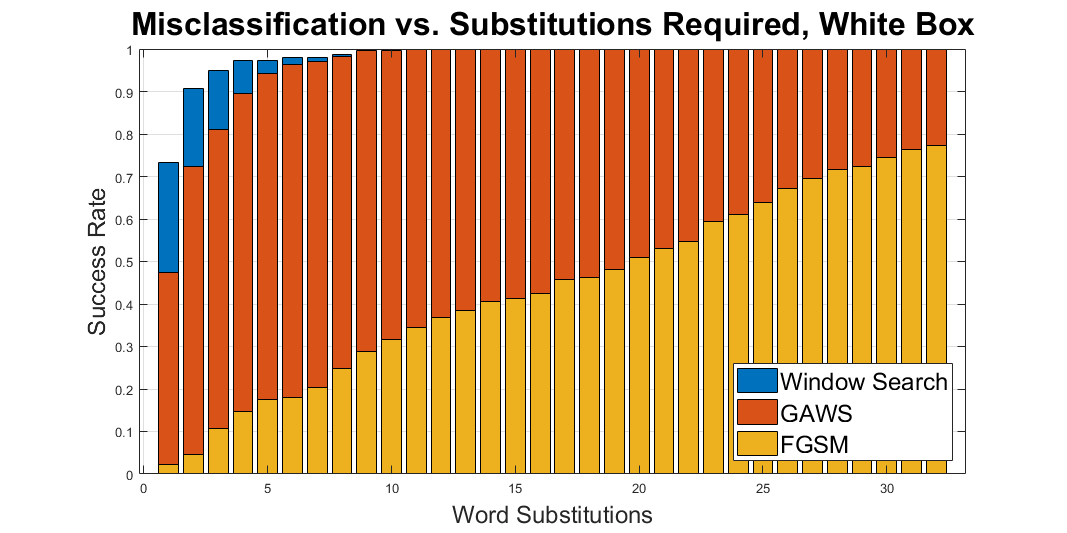
\includegraphics[width=\textwidth]{images/cdf_white.png}
    \caption{The x-axis represents the number of word substitutions used to change the fraction of samples represented by the y-axis.}
    \label{fig:whitepmf}
\end{figure}

\end{document}
